\documentclass[12pt, a4paper, oneside]{book}
\usepackage[hidelinks]{hyperref}
\usepackage[slovak]{babel}
\usepackage{epsfig}
\usepackage{epstopdf}
\usepackage[chapter]{algorithm}
\usepackage{algorithmic}
\usepackage{listings}
\usepackage{amsmath}
\usepackage{amssymb}
\usepackage{graphicx}
\usepackage{multirow}
\usepackage{color}
\usepackage{url}
\usepackage[utf8]{inputenc}
\usepackage[T1]{fontenc}
\usepackage{setspace}
\usepackage{tabularx}
\usepackage{textcomp}
\usepackage{caption}
\usepackage{natbib}
\usepackage{pdfpages}

% TODO NOTES
\usepackage{todonotes}
%\usepackage[disale]{todonotes}
\usepackage{xcolor}
\usepackage[normalem]{ulem}
\usepackage{soul}

%%% TODO Notes
\newcommand{\assignment}[2][]{\todo[caption={},inline,bordercolor=green!67!yellow!75!black!50,color=green!67!yellow!25,size=\footnotesize,#1]{#2}}
\newcommand{\overview}[2][]{\todo[caption={},inline,color=blue!85!green!25,bordercolor=blue!85!green!50!black!50,size=\footnotesize,#1]{#2}}
\newcommand{\minor}[2][]{\todo[caption={},color=gray!30,bordercolor=gray,inline,size=\footnotesize,#1]{#2}}
\newcommand{\cutting}[2][]{\todo[color=yellow!30,bordercolor=yellow!50!black!50,inline,size=\footnotesize,#1]{#2}}
\newcommand{\bigassignment}[2][]{\todo[inline, caption={Big assignment},
    color=green!40, #1]{\begin{minipage}{\textwidth-4pt}#2\end{minipage}}}
\newskip\movedskip
\newcommand{\movespaceafter}[1]{%
    \movedskip=0pt%
    \ifhmode\ifdim\lastskip=0pt\else\movedskip=\lastskip\unskip\fi\fi
    #1\ifdim\movedskip=0pt\else\hskip\movedskip\fi
    \ignorespaces}
\newcommand{\reviewnote}[3][]{%
  \movespaceafter{\todo[inline,color=yellow!75!white,linecolor=yellow!85!black,#1]
      {\textsf{\bfseries Review #2:} \ignorespaces#3\par}}%
}
%\newcommand{\comment}[3][]{%
%  \movespaceafter{\todo[color=green!40,#1]
%      {\textsf{\bfseries #2:} \ignorespaces#3\par}}%
%}

\definecolor{mossgreen}{HTML}{146614}
\newcommand{\del}[1]{\color{red}\sout{#1}\color{black}\@}
\newcommand{\ins}[1]{\color{mossgreen}\uwave{#1}\color{black}\@}
\newcommand{\sug}[2]{\del{#1}\ins{#2}}

\newcommand{\UP}{$\uparrow$}
\newcommand{\DOWN}{$\downarrow$}
\newcommand{\UD}{$\updownarrow$}




\setstretch{1.5}
%\renewcommand\baselinestretch{1.5} % riadkovanie jeden a pol

% pekne pokope definujeme potrebne udaje
\newcommand\mftitle{Sémantické publikovanie spravodajských dát}
\newcommand\mftitlen{o bezpečnostných hrozbách}
\newcommand\mfthesistype{Diplomová práca}
\newcommand\mfauthor{Bc. Matej Rychtárik}
\newcommand\mfadvisor{doc. RNDr. Martin Homola, PhD.}
\newcommand\mfplacedate{Bratislava, 2021}
\newcommand\mfuniversity{UNIVERZITA KOMENSKÉHO V BRATISLAVE}
\newcommand\mffaculty{FAKULTA MATEMATIKY, FYZIKY A INFORMATIKY}
\newcommand{\sub}[1]{$_{\text{#1}}$}
\newcommand{\reference}[1]{č.~\ref{#1}}
\newcommand{\imageHeight}{150px}

\ifx\pdfoutput\undefined\relax\else\pdfinfo{ /Title (\mftitle) /Author (\mfauthor) /Creator (PDFLaTeX) } \fi

\begin{document}

\frontmatter

\thispagestyle{empty}

\noindent
\begin{minipage}{\textwidth}
\begin{center}
\textbf{\mfuniversity \\
\mffaculty}
\end{center}
\end{minipage}

\vfill
\begin{figure}[!hbt]
	\begin{center}
		
\includegraphics{images/logo_fmph}
		\label{img:logo}
	\end{center}
\end{figure}
\begin{center}
	\begin{minipage}{0.8\textwidth}
		\centerline{\textbf{\Large\MakeUppercase{\mftitle}}}
		\smallskip
		\centerline{\mfthesistype}
	\end{minipage}
\end{center}
\vfill
2021 \hfill
\mfauthor
\eject 
% koniec obalu

\thispagestyle{empty}

\noindent
\begin{minipage}{\textwidth}
\begin{center}
\textbf{\mfuniversity \\
\mffaculty}
\end{center}
\end{minipage}

\vfill
\begin{figure}[!hbt]
\begin{center}

\includegraphics{images/logo_fmph_dark}
\label{img:logo_dark}
\end{center}
\end{figure}
\begin{center}
\begin{minipage}{0.8\textwidth}
\centerline{\textbf{\Large\MakeUppercase{\mftitle}}}
\smallskip
\centerline{\mfthesistype}
\end{minipage}
\end{center}
\vfill
\begin{tabular}{l l}
%Registration number: & 40a99bd8-3cb6-4534-9330-c7fd9b5e5ca4 \\
Študijný program: & Aplikovaná informatika\\
Študijný odbor: & 2511 Aplikovaná informatika\\
Školiace pracovisko: & Katedra aplikovanej informatiky\\
Školiteľ: & \mfadvisor
\end{tabular}
\vfill
\noindent
\mfplacedate \hfill
\mfauthor
\eject 
% koniec titulneho listu

%\thispagestyle{empty}
%\includegraphics[width=\textwidth]{images/zadanie}
%\vfill
%\eject
% koniec zadania

\thispagestyle{empty}

%\includepdf[pages=1,scale=1]{zadanie.pdf}

{~}\vspace{12cm}

\noindent
\begin{minipage}{0.25\textwidth}~\end{minipage}
\begin{minipage}{0.75\textwidth}
Čestne prehlasujem, že túto diplomovú prácu som vypracoval samostatne len s použitím uvedenej literatúry a za pomoci konzultácií u môjho školiteľa.
\newline \newline
\end{minipage}
\vfill
~ \hfill {\hbox to 6cm{\dotfill}} \\
\mfplacedate \hfill \mfauthor
\vfill\eject 
% koniec prehlasenia

\chapter*{Poďakovanie}\label{chap:thank_you}
Touto cestou by som sa chcel v prvom rade poďakovať môjmu školiteľovi doc. RNDr. Martinovi Homolovi, PhD. za jeho cenné rady a usmernenia, ktoré mi veľmi pomohli pri riešení tejto diplomovej práce. 
\vfill\eject 
% koniec podakovania

\chapter*{Abstrakt}\label{chap:abstract_sk}


\chapter*{Abstract}\label{chap:abstract_en}

% koniec abstraktov

\tableofcontents

\mainmatter

% treba este prejst dokument ci je kod spravne formatovany
\chapter{Úvod}\label{chap:intro}
Nejaky strucny uvod do problematiky

\part{Prehľad problematiky}
\chapter{Sémantický web}
Semantický web \cite{semantic} poskytuje spoločný framework, ktorý umožňuje zdieľanie a opätovné použitie údajov v rámci aplikácií. Štandardy podporujú spoločné dátové formáty a protokoly, kde najpodstatnejším je Resource Description Framework (RDF). Prvýkrát pojem Semantický web zaviedol Tim Berners-Lee a popisoval "dátový web", ktorý môže byť strojovo čitateľný. Zámerom je zvýšiť použiteľnosť webu a jeho prepojených zdrojov vytvorením sémantického webu. Semantický web má vrstvovú štruktúru ako si môžeme všimnúť na obrázku 2.1. Jednotlivé údaje sú potrebné až vo vyšších vrstvách. XML vrstva zaručuje, že môžeme spájať Semantický web s inými normami založenými napríklad na XML, ktorá je rozšírená a podporovaná a RDF dáta sa v nej dajú dobre prenášať, spracovávať a uchovávať. RDF a RDFS vrstva definuje typ zdrojov. Ontologická vrstva podporuje vývoj ontológií, vďaka ktorým môžeme definovať vzťahy medzi rôznymi pojmami.

\assignment{MH: \UP Toto trochu povrchne: (1) Ucelom SW nie je vyssia pouzitelnost webu (to je nepresne), ale je to lepsia pristupnost informacii publikovanych na webe pre strojove spracovanie. (2) Ak chces popisovat vrstvy SW podla tohto diagramu, bolo by dobre keby si popisal vsetky vrstvy -- U XML by som sa obmedzil na to, ze je to proste dobry format pre textovu reprezentaciu dat v suboroch a pre ich vymenu medzi softvermi -- toto vsak uz je dnes prekonane, uz vymiename SW data aj ako JSON, embedujeme ich do HTML5 (chcelo by to poznamku) -- O RDF a RDFS si vlastne nic uzitocne (z coho citatel nieco vyrozumie) nepovedal -- no a ostatne vrstvy si uplne preskocil\\
MH: Toto si menil? Zda sa mi, ze trochu asi aj ano, ale o tych dalsich vrstvach si nic nenapisal}

\begin{figure}
\makebox[\textwidth]{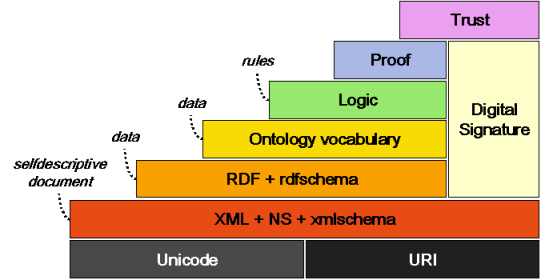
\includegraphics[scale=0.7]{images/semantic_web}}
\label{fig:semantic_web}
\caption{Semantic Web - vrstvy.\\Zdroj: \cite{semanticweb}}

\end{figure}


Text uvedený nižšie popisuje niekoľko technológií, ktoré sú potrebné pre tvorbu sémantického webu.

\section{Linked Data}

\assignment{MH: \DOWN Tato sekcia je celkom fajn ale chybalo mi trochu
premostenie od SW -- linked data bola iniciativa, ze ked uz SW formaty mame,
podme v nich aj data zverenjnovat}

\minor{MH: Inak ked uz si sa rozhodol pisat po slovensky, mal by si pouzivat aj
slovensku terminologiu (co je celkom peklo) -- ale teda Linked Data su
\emph{prepojene data}, LD network je \emph{siet prepojenych dat} -- ludia to takto pouzivaju}

Linked Data \cite{linkeddata} je metóda zverjňovania štrukturovaných dát. Ich hlavným cieľom je poprepájať existujúce databázy (primárne písané v RDF formáte), medzi rôznymi údajmi a umožniť ľuďom zdielať štrukturované dáta na webe pomocou HTML. Časť vízie do budúcna je, aby sa Internet stal globálnou databázou. Princípy Linked Data prvýkrát načrtol Tim Berners-Lee. Popísal 4 pravidlá pre zverejňovanie dát na webe:
\begin{enumerate}
  \item používať URI ako názvy objektov, ktoré sú identifikátormi informácie, jej umiestnenia a ďalších vlastnotí,
  \item používať HTTP URI, aby si ich ľudia vedeli pozrieť,
  \item uvádzať informácie o tom, čo názov identifikuje pri vyhľadávaní pomocou otvorených štandardov, ako sú napríklad RDF alebo SPARQL,
  \item pri publikovaní údajov na webe, zahrnúť odkazy aj na iné URI, aby sa dalo objavovať viac vecí.
\end{enumerate}
Sú známe aj ako Linked Data princípy.

\assignment{MH: Tu mi chyba informacia, ze sa tato inciativa ujala, a ze vdaka
tomu vznikla na webe tzv. siet prepojenych dat, ktora obsahuje obrovske mnozstvo
datovych zdrojov a nieco viac o tej sieti.}


\section{Resource Description Framework (RDF)}

RDF \cite{rdf} je štandartný model na zakódovanie metadát a ďalších informácií. Je to taktiež formát, ktorý bol navrhnutý a štandardizovaný na reprezentáciu dát pre sémantický web. Zdroje týchto dát sú väčšinou webové zdroje, ktoré môžu byť čokoľvek, napríklad dokumenty, ľudia, fyzické objekty, atď. Taktiež poskytuje spoločný framework na vyjadrenie informácií a možnosť zdieľať ich medzi softvérmi, bez straty ich hodnoty. Dáta sa uchovávajú v Triple Store databázach, ktorých formát je striktne daný. Výhodou je, že dáta môžu byť spracované aj softvérmi, pre ktoré dané dáta neboli vytvorené.

\assignment{MH: \UP Na co RDF sluzi sa uz citatel dozvedel v skorsich castiach
(ked to tam lepsie ozrejmis). Niektore veci, ktore tu \UP pises su nepresne
(napr. to o tych metadatach a ``dalsich informaciac'' alebo o zdrojoch. Tiez o Triple Stores predbiehas, budes o tom pisat neskor\ldots Asi by som to tu skratil a len by som nadviazal, ze RDF je zakladny datovy format pre SW a tu ho popiseme\ldots}

\assignment{MH: \DOWN Zvysok ide dobrym smerom, je to presne to, co by som si predstavoval, ze tu budes pisat, len by som to chcel vidiet mozno trochu pomenej, podrobnejsie, systmatickejsie prebrate\ldots Na vacsom priestore, mozno postupne ten priklad budovat\ldots Vysvetlit na nom vsetky zakladne moznosti RDF}


RDF súbor je taký dokument, ktorý ukladá RDF grafy do špecifického formátu serializácie pre RDF, ako sú napríklad N-Triple, TURTLE, RDF/XML a mnohé ďalšie. RDF bol postavený na myšlienke vytvárať údaje vo forme predmet-predikát-objekt, ktorý sa volá "triple", ďalej len trojica. Trojica je základná stavebná jednotka akejkoľvek množiny dát zapísaných v RDF. Tieto údaje sú reprezentované ako orientované grafy. Predmet a objekt predstavujú vrcholy a predikát je orientovaná hrana medzi nimi. Predmet môže byť použítý aj ako objekt v inej trojici. Týmto spôsobom sa trojice prepájajú a vzniká z nich grafová databáza. Predmet je vždy definovaný ako URI a popisuje zdroj informácie. Objekt môže byť taktiež nejaké URI popisujúce zdroj, ale taktiež to môže byť primitívna hodnota ako napríklad string, integer, date, atď. Predikát popisuje, aký vzťah alebo rola medzi predmetom a objektom existuje. Predikát je vždy reprezentovaný ako URI, ktoré pochádza z ontolológií (kolekcie viacerých URI).


Na uľahčenie ukladania a čitateľnosti dát sa využívajú takzvané prefixy, ktoré sú preddefinovaním základných URI, do ktorých sa dodáva zvyšná hodnota URI pomocou dvojbodky, ako je to uvedené v nasledujúcom príklade a graficky znázornené v obrázku 2.2.
\begin{verbatim}
@prefix  rdf: <http://www.w3.org/1999/02/22-rdf-syntax-ns> .
@prefix	 dbr: <http://dbpedia.org/resource/> .
@prefix 	 dbo: <http://dbpedia.org/ontology/> .
@prefix  dbp:<http://dbpedia.org/property/> .

dbr:Bratislava dbo:highestPlace dbr:Devínska_Kobyla .
dbr:Bratislava rdf:type dbo:City .
dbr:Bratislava dbo:country dbr:Slovakia .
dbr:Devínska_Kobyla dbo:locatedInArea dbr:Slovakia .
dbr:Slovakia dbp:drivesOn "right" .
dbr:Slovakia dbo:longName "Slovak Republic"@en .
\end{verbatim}

\begin{figure}[h]
\makebox[\textwidth]{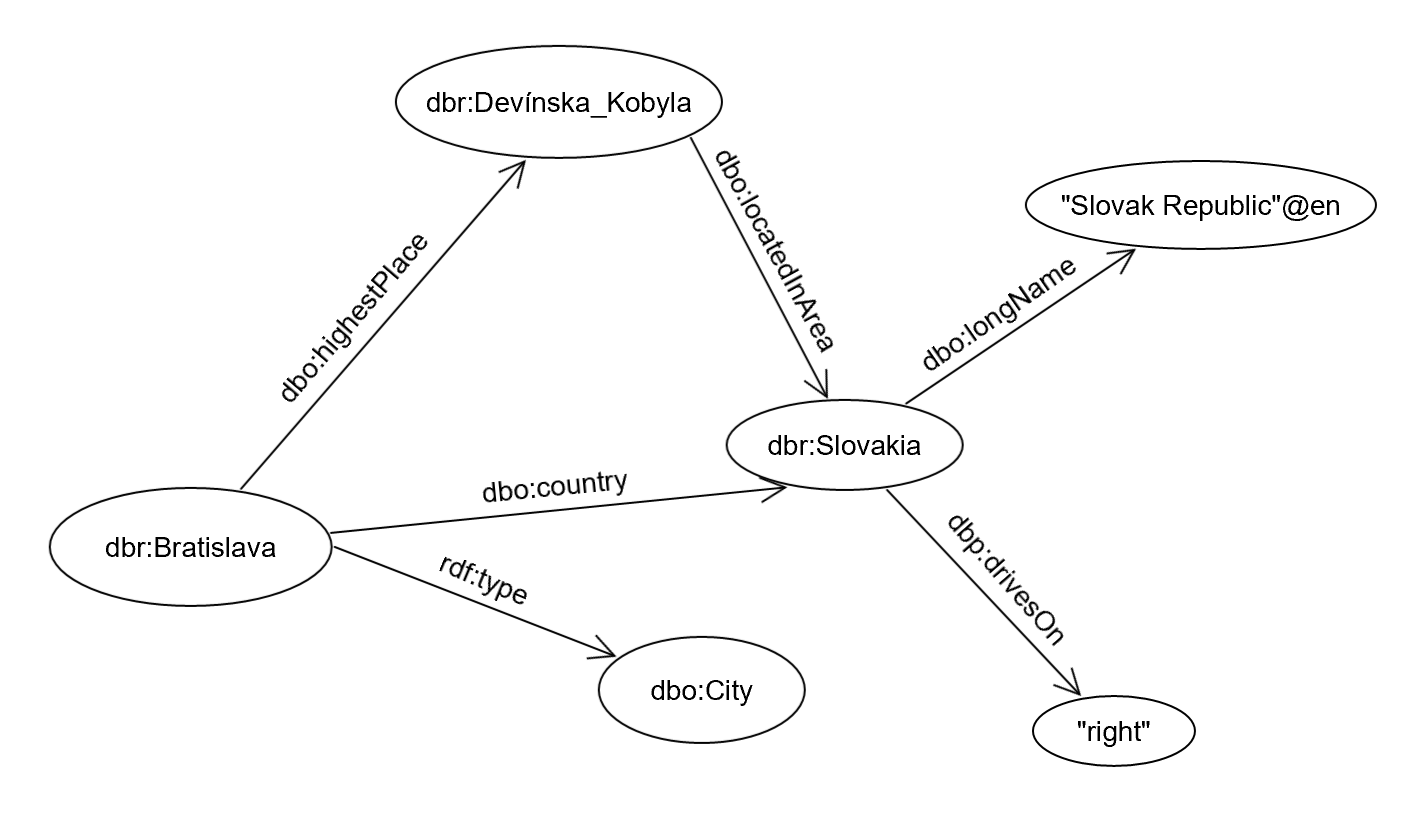
\includegraphics[keepaspectratio=true,scale=0.7]{images/triple_example}}
\label{fig:semantic_web}
\caption{Príklad grafovej databázy.}
\end{figure}


\chapter{Ontológie}

\assignment{MH: Predpokladam, ze o ontologiach budeme pisat o znacny kus viac a
podrobnejsie\ldots Mozes vychadzat z mojej prednasky ale tiez napr z uvodnej
kapitoly \emph{Handbook on Ontologies}}

\overview{MH: Pozn.\ k strukture prace: Bolo by lepsie, keby \emph{Prehlad problematiky} bola cast \texttt{\textbackslash{}part\{\}}, \emph{Semanticy web} samostatna kapitola\texttt{\textbackslash{}chapter\{\}}, no a potom si myslim, ze \emph{Ontologie} by tiez mali mat vlastnu kapitolu, ktora bude nasledovat hned po SW. Tretou kapitolou by potom mohol byt prehlad ontologii z oblasti bezpecnosti, co by uz do prehladu problematiky mohlo aj stacit}


Výraz ontológia \cite{ontologies} pochádza z gréckeho slova kde '\textit{ontos}' znamená existencia a '\textit{logos}' znamená veda. Ontológia v informatike je uceleným popisom pojmov v určitej oblasti záujmu. Obsahuje určitú klasifikáciu údajov do hierarchicky usporiadaných kategórií a množinu odvodzovacích pravidiel, pomocou ktorých je možné z faktov odvodiť nové skutočnosti. Prostredníctvom ontológií je možné vytvárať spojenia v prirodzenom jazyku, vykonávať analýzu údajov a sprostredkovať výhody webu obohateného o sémantiku. 

\assignment{MH: nerozumiem co myslis pod \uv{vytvárať spojenia v prirodzenomjazyku} a tiez tvrdenie \uv{sprostredkovať výhody webu obohateného o sémantiku} je velmi abstraktne neviem celkom prist na to co si tym asi myslel}

\section{Základné pojmy}
Ontológia sa skladá zo základných stavebných prvkov \textit{Trieda}, \textit{Entita}, \textit{Atribút}, \textit{Väzba}. 


\textbf{Triedy} alebo typy definujú skupiny alebo množiny objektov. Triedy majú hierarchickú štruktúru zloženú z ich podtried. Každá podtrieba spĺňa vlastnosti nadtriedy a môže byť rozšírená o vlastné vlastnosti.


\textbf{Entity} sú individuálne inštancie nejakej nami zadefinovanej triedy. Ak by sme mali entitu \textit{Jablko}, a triedy \textit{Ovocie} a \textit{Jedlo}, kde \textit{Ovocie} je podtriedou \textit{Jedlo}, tak nám z ontológie vyplýva, že ak je entita \textit{Jabllko individuálnou inštanciou triedy \textit{Ovocie}, tak je aj individuálnou inštanciou triedy \textit{Jedlo}.}

\minor{MH: $\uparrow$ \emph{Jablko} nie je velmi dobry priklad na entitu, kedze vacsinou ho uvazujeme ako triedu (a teda podtriedu triedy Ovocie)}


\textbf{Atribúty} sú vlastnosti \textit{Tried} a \textit{Entít} a môžu niesť rôzne informácie o danom objekte. \textit{Atribúty} môžu mať rôzne hodnoty, ako reťazec, číslo, dátum, pravdivostnú hodnotu alebo inú premennú. Ak by sme si zobrali predchádzajúcu entitu \textit{Jablko}, jej číselná vlastnosť môže byť napríklad mesiac kedy sa oberá alebo jej reťazcová vlastnosť farba.

\assignment{MH: $\uparrow$ Je pomerne nezvycajne aby mali atributy ako hodnotu inu premennu}

\textbf{Väzby} sú najpodstatnejšou súčasťou ontológie. Poskytujú prepájanie jednotlivých objektov tried. Je to jednosmerné spojenie, ktoré určuje vzťah, v akom sú dve dané triedy. Tým vznikne trojica \textit{trieda:vzťah:trieda}, ktorá sa nazýva triplet. Medzi triplet sa radí aj trojica \textit{trieda:atribút:hodnota}. Väzby sa zvyknú definovať aj inverzne.

\assignment{MH: $\uparrow$ nazov \emph{vazby} je velmi exoticky. Ak ti ide o object properties, pouzil by som slovo \emph{vztahy}.}
\assignment{MH: $\uparrow$ to co je \emph{triplet} by si mal zadefinovat vyssie, kde pises o RDF.}
\assignment{MH: $\uparrow$ Co su \uv{objekty tried}? Kusok vyssie si si pre objekty zvolil nazov \emph{entity}, mal by si ho teda pouzivat. Ak ti ide o vztahy medzi triedami, ako napr. vztah podtriedy a nadtriedy, v RDF je to sice vyjadrene pomocou vlasntosti, ale z logickeho hladiska to chapeme ako \emph{axiom}}

Ontológia má veľa vlastností, ktoré musia byť dodržané. Každý prvok musí byť jasne indetifikovateľný. Taktiež zakazuje zapisovanie duplicitných dát, čo nám zaobstará vlastnosť efektívneho ukladania informácií, kde to môže nie len uľahčiť vyhľadávanie ale aj obsah pamäti na disku. 

\assignment{MH: $\uparrow$ Neviem, ci zrovna tieto vlastnosi ontologii su tie najpodstatnjsie, a teda treba ich spominat na tomto mieste.}

\section{Využitie ontológií}

\minor{MH: $\downarrow$ Asi by som sa neodvazoval tvrdit to co pises v prvej vete. Ak zoberieme ako ranne vyuzitie napr. SNOMED, nie je to pravda, kedze sa vyuzival v medicinskej praxi. S druhou vetou mozno nesuhlasit. Kto je bezny pouzivatel? Nikomu takemu sa nerozsirila do pocitaca nejaka ontologia (ze by o tom vedel)\ldots}
Ontológie sa začali využívať najmä v organizáciách, ktoré sa šoecializovali na umelú inteligenciu. Neskôr sa to rozšírilo aj do počítačov bežných používateľov. Napríklad firma Amazon používa ontológie na kategorizovanie tovaru v ich elektronickom obchode.


Na zápis týchto ontológií sa používa niekoľko jazykov, kde najznámejším je asi Resource Description Framework (RDF), ktorý je rpimárne určený na využitie vo webových stránkach, pre hľadanie informácií strojmi. Ontológie si našli uplatnenie aj v medicínskej oblasti a to napríklad SNOMED, čo je najväčším viacjazyčným medicínskym slovníkom na svete. 

\assignment{MH: $\uparrow$ Tu chces asi pisat o vyuziti ontologii, takze zmienka o jazyku RDF sem nepatri, navyse RDF nie je jazyk na zapis ontologii (tym je RDFS) a o RDF su uz pisal vyssie}


Taktiež sa s ním stretávame každodenne pri vyhľadávaní na stránke Google, kde ako bočný panel sú zobrazené informácie o vyhľadávanom objekte (obrázok nižšie). Tieto dáta je možné zobraziť preto, lebo výsledkom takéhoto panelu je vyhľadávanie informácií na webovej stránke, ktorá obsahuje sémantické dáta.

\minor{MH: $\uparrow$ SNOMED a Google spominas dobre, a v druhom pripade si nespomenuk ziadnu ontologiu a pritom ju dobre pozname (Schema.org)}

Na získavanie dát zo sémantických webov a z RDF úložísk sú využívane SPARQL dopyty. Syntax jazyku SPARQL je veľmi podobná klasickému SQL jazyku, kde aj SPARQL umožňuje okrem dopytovania aj vkladanie, editáciu a vymazávanie dát.

\assignment{MH: $\uparrow$ toto mi sem opat nesedi, zrejme tomu chces venovat nejaku kratku podsekciu skor v predchadzajucej kapitole (?)}


\section{Ciele ontológie}
Zadefinovanie a zdieľanie jednotného zápisu informácií pre danú doménu. Ak napríklad viac stránok využíva na popis pojmov takúto zadefinovanú ontológiu, vedia boti získať a vyhľadávať viac dát o hľadanej informácii.


Taktiež je jej cieľom opätovné použitie ontológie, napríklad ak máme dobre zadefinovanú ontológiu, môžu ontologický inžinieri doplniť do našej ontológie ďalšie vlastnosti a tým by základ ontológie bol rovnaký ale bol by rozšírený o určité dáta, podľa potreby ontologických inžinierov.


\assignment{MH: $\uparrow$ Tuto cast mozno lespie najko pouzit v uvode predch. casti (?)}

\section{Syntax ontológií}
\textbf{MAM SPRAVIT AJ TOTO?}

\assignment{MH: Kedze cela Tvoja praca je o ontologiach a budes ich zrejme nejako zapisovat mozno by si mohol nieco povedat aj o jazykoch na zaspis ontologii, minimalen apson o jednom, s ktorym budes pracovat dalej (cize zrejme OWL)}

\chapter{Existujúce ontologické riešenia v oblasti bezpečnosti}
STRUCNY POPIS KAPITOLY

\section{CTI model}
TEN BY SOM MOZNO ZAHRNUL SEM CI?

\section{UCO}
\minor{MH: Lepsie ked v nadpisoch nebudes pouzivat skratky}
\assignment{MH: Chybaju tu akekolvek referencie}

Unified Cybersecurity Ontology alebo skrátene UCO je rozšírením pôvodného projektu Intrusion Detection System (IDS), ktorého tvorcom je rovnaká skupina. Spája viaceré bežne dostupné bezpečnostné štandardy používané v kybernetickej bezpečnosti. Prevažne pokrýva STIX, ktorý je najväčším a najkomplexnejším štandardom, pokrývajúcim najväčšiu časť kybernetickej bezpečnostnej domény ale taktiež poskytuje iné relevatné štandardy ako CVE4, CCE5, CVSS6, CAPEC7, CYBOX8, KillChain9 a STUCCO10.

\minor{MH: $\uparrow$ Zrejme muslis \emph{pokryva} ine relevantne standardy? Ak nie, nerozumiem, v akom zmysle ich poskytuje?}

Aj keď je STIX najkomplexnejším štandardom a zjednocuje všetky informácie o kybernetických hrozbách, má tieto dáta uložené v XML súboroch, takže nepodporuje výhody uvažovania v ontológiách, čo UCO poskytuje.

\minor{MH: $\uparrow$ \emph{uvazovanie v ontologiach} nie je spravny slovensky vyraz pre reasoning -- skus napr. \emph{inferencia}}

Okrem týchto štandardov obsahuje aj mapovanie na všeobecné \del{svetové} databázy ako sú Google Knowledge Graph, DBPedia a Yago. Vďaka týmto mapovaniam je možné mať prístup k verejným databázam r rôznych domén záujmu.


Základnými triedami, využívanými v UCO sú: 
\begin{itemize}
\item \textit{Means} -- Čo je zamýšľané daným útokom.
\item \textit{Consequences} -- Dôsledky útoku.
\item \textit{Attack} -- Typ útoku.
\item \textit{Attacker} -- Kto je inicitorom daného útoku.
\item \textit{Attack-Pattern} -- Vzorec útoku, podľa ktorého je útok riadený.
\item \textit{Exploit} -- K čomu útok slúži.
\item \textit{Exploit Target} -- K čomu slúži cieľ alebo výsledok útoku.
\item \textit{Indicators} -- Indikátor útoku.
\end{itemize}
Každá z týchto tried je mapovaná na už reálne existujúcu triedu v niektorom z vyššie uvedených štandardov, prevažne na STIX schému.


Ontológia UCO umožňuje analytikom zachytávať špecifické vedomosti o kybernetickej bezpečnosti pomocov termínov a tried z ontológie a taktiež umožňuje písať pravidlá, ktoré sa môžu použiť na odvodenie nových poznatkov.


Vývojári extrahovali dáta z National Vulnerability Database (NVD), ktorá je uložená v XML súboroch. Potom boli namapované na triple store DBPedia a dáta boli uložené na FUSEKI server, ktorý podporuje dopytovanie z rôznych zdrojov rovnako ako ich odvodzovanie.
\section{ICAS}

\section{•}


\backmatter

\nocite{*}
\bibliographystyle{alpha}
\bibliography{references}

\listoffigures

\end{document}
